\chapter{Introduction}\label{ch:introduction}
The Lego Group began manufacturing the lego bricks in 1949. 
Assume that you work in a company producing Simpson figures made by Dublo brucks.
\begin{enumerate}
\item The figures come in two sizes. One size consisting of 3x1 (or 2x1 for Maggie) Dublo bricks and one consists of 3x4 (or 2x4 for Maggie) brick.
\item A customer can order a set of figures
\end{enumerate}

The Dublo bricks are located randomly (but not
overlapping) on a table next to a robot.
\begin{enumerate}
\item A camera is located above the table so that all the
bricks are within the view of the camera.
\item Your task is to design a system which can produce
the Simpson figures. 
\end{enumerate}

\begin{figure}[hb]
  \centering
  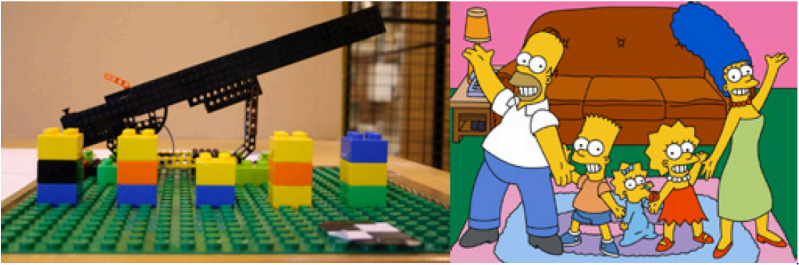
\includegraphics[width=4in]{figures/simpsonLegoBricks.png}
  \caption[Simpsons figures Lego Bricks]
   {A illustration of the simpsons figures with Lego Duplo Bricks}
\end{figure}

This involves among other things:
\begin{enumerate}
\item Identifying which bricks are located on the table.
\item Identifying the location of the bricks (e.g. the location of a
black Dublo brick needed to build Homer)
\item Determine the associated cost of each solution and the
cheapest solutions.
\item Grasping the bricks by means on a robot.
\item Mounting the bricks on a plate or on top of other bricks
\item Selecting the sequence in which you want to pick/place
the bricks and build the figures
\end{enumerate}


